\subsection{2. 架构}\label{architecture}

\subsection{2.1. 概览}\label{overview}

DeepSeek-V4.1-Flash 是一个多模态混合专家（MoE）Transformer，以图像和文本作为输入，并以自回归方式生成文本。其语言主干由 40 层因果 Transformer 层组成，组织为一个 20 层因果编码器后接一个 20 层解码器。除前两层仅使用滑动窗口注意力（SWA）外，每一层都同时包含全局注意力和滑动窗口注意力。视觉编码器和 MLP 投影器将图像转换为视觉嵌入，与文本嵌入联合处理，多模态数据从语言模型预训练之初即被纳入。总体而言，DeepSeek-V4.1-Flash 拥有 552B 主干参数和 196B Engram 参数，预填充阶段每个 token 激活 8B 参数，解码阶段激活 16B 参数。图 3 展示了 DeepSeek-V4.1-Flash 的整体架构。

因果编码器--解码器（CED）架构与压缩稀疏注意力 2（CSA2）



共同解决长上下文推理中的互补性成本。CED 从编码器输出构建解码器的全局键值（KV）缓存，使大多数提示词 token 可以绕过完整的解码器计算，同时保留逐层局部的滑动窗口注意力。这几乎将预填充计算量减半，降低了在上下文不断增长的智能体工作负载中处理新输入或未缓存输入的成本。CSA2 跨层共享全局 KV 以降低缓存存储，并复用稀疏选择以减少索引工作量。在解码器中，分层稀疏索引器（Hierarchical Sparse Indexer）将后续索引器限制在由更早的索引器选出的候选池内，从而进一步减少每个查询需要计分的条目数量。

我们保留了 DeepSeekMoE（Dai et al., 2024）的共享专家和细粒度路由专家，并为图像和文本 token 引入了模态特定的负载均衡（Wang et al., 2024a）。Single-Pass mHC（Xie et al., 2026）改进了残差流混合方式，以实现更高效的核融合，Engram（Cheng et al., 2026b）则增加了可稀疏访问的条件记忆。我们在主干预训练期间省略了 MTP 模块，并使用 DSpark（Cheng et al., 2026a）进行推测解码。我们在主干预训练阶段之后单独训练 DSpark。此外，我们将主 KV 缓存压缩为 FP4，以进一步减少存储开销。以下各节介绍这些组件及相应的优化改动。

\subsection{2.1.1. 多模态架构}\label{multimodal-architecture}

多模态输入通路由一个视觉编码器和一个 MLP 投影器组成。对于每张输入图像，视觉编码器都会生成一个视觉特征的空间网格。随后，一个 3 $\times$ 3 的 pixel-unshuffle 操作沿通道维度重排每个局部邻域，在 MLP 投影器将特征映射到语言主干的隐藏维度之前降低空间分辨率。最后，得到的视觉嵌入会被插入到输入嵌入序列中对应图像 token 的位置，并由语言主干与文本嵌入联合处理。

DeepSeek-ViT 我们从零开始训练了一个名为 DeepSeek-ViT 的视觉编码器，使其能够原生处理不同分辨率的图像。我们在 Vision Transformer（Dosovitskiy et al., 2021）架构的基础上构建 DeepSeek-ViT，并做了若干修改。为容纳任意分辨率的输入，我们用 2D-RoPE 替换了标准的绝对位置嵌入。为使 ViT 更贴近 LLM 的设计原则，我们将 patch 嵌入层的卷积替换为线性投影，以确保与 Muon 优化器兼容。我们还采用 RMSNorm（Zhang and Sennrich, 2019）进行归一化，并使用 SwiGLU（Shazeer, 2020）作为激活函数。在将视觉特征送入 LLM 之前，我们应用一个 3 $\times$ 3 下采样的 pixel-unshuffle 操作，将视觉 token 数量减少为原来的九分之一，从而有效支持高达约 1344 $\times$ 1344 像素的输入分辨率。

多模态 MoE 的无辅助损失负载均衡 图像 token 与文本 token 表现出不同的表征分布，可能在 MoE 中诱发不同的专家路由偏好。因此，平衡它们的总体负载可能会掩盖模态特定的不均衡。为解决这一问题，我们扩展了无辅助损失负载均衡（Wang et al., 2024a），为文本和图像 token 分别维护独立的按专家修正偏置。在路由过程中，每个 token 使用与其模态关联的修正偏置进行专家选择，同时保留原始路由分数用于对所选专家输出进行加权。每个训练步骤之后，两组偏置根据各自的专家负载独立更新。这一设计平衡了每种模态内部的专家利用率，有助于稳定高效的多模态训练。



\subsection{2.2. 因果编码器-解码器（CED）}\label{causal-encoder-decoder-ced}

在智能体工作流中，频繁的工具调用会产生大量预填充请求，当 KV 缓存未命中时会带来严重的计算开销。为缓解这一预填充瓶颈，我们提出了因果编码器-解码器（CED）架构，其灵感来自 YoCo（Sun et al., 2024）。YoCo 通过允许上层一半的层直接共享下层一半的层生成的 KV 缓存来减少预填充计算。在此基础上，CED 引入了一系列结构性改进，以同时提升整体 KV 缓存容量和 KV 生成的计算深度。因此，CED 在保持与基线相当性能的同时，成功将预填充计算量减少了近一半。

对于全局注意力，CED 将 Transformer 的底部 \(L / 2\) 层视为因果编码器。对于上层一半的层（即解码器，\(l > L / 2 )\) ），KV 条目并非直接来自它们各自的隐藏状态 \(H _ { l } .\) 。相反，它们是使用随层变化的投影权重 \(( \dot { W } _ { l } ^ { K V }\) 和 \(W _ { l } ^ { Z } )\) 从第 \(( L / 2 )\) 层的隐藏状态 \(H _ { L / 2 }\) 投影得到的：

\[
C _ { l } = H _ { L / 2 } W _ { l } ^ { K V } , \quad Z _ { l } = H _ { L / 2 } W _ { l } ^ { Z } , \quad l > \frac { L } { 2 } ,\tag{1}
\]

其中 $C$ 与 $Z$ 分别表示 KV 条目及其对应的压缩权重。这一设计使 CED 在预填充阶段只需计算前一半的层，便能以极小的计算量获得上层的全局 KV 缓存。

对于滑动窗口注意力（SWA），CED 在所有层中保持传统的逐层计算。具体而言，对于任意层 $l$，局部键和值直接从当前层的隐藏状态 \(H _ { l } .\) 得出。这一设计有效增加了局部 KV 生成的计算深度。然而，保持这种逐层计算需要一次 SWA 重放（replay）过程。在预填充阶段，为解码器计算 SWA KV 缓存需要额外处理 \(n _ { \mathrm { w i n } } \times L / 2\) 个 token（其中 \(n _ { \mathrm { { w i n } } }\) 表示窗口大小）。对于每轮提示都很短的多轮交互，解码器中的这一计算开销变得不可忽略。幸运的是，先前的工作（Chen et al., 2025）已经表明，SWA 的实际有效感受野远小于理论上的 \(n _ { \mathrm { w i n } } \times L / 2\)。受此启发，我们引入了 Decoder SWA Bounded Replay，它只为 SWA 计算预填充提示中最后 \(n _ { \mathrm { w i n } }\) 个 token，从而显著降低计算成本。更多细节见第 3.2.2 节。

总体而言，对于序列长度 \(N \gg n _ { \mathrm { w i n } } ,\) CED 将预填充复杂度从 \(O ( N L )\) 降低为 \({ \cal O } ( N L / 2 + n _ { \mathrm { w i n } } \times L / 2 ) \approx { \cal O } ( N L / 2 )\)，实际将整体计算量减半。

\subsection{2.3. 压缩稀疏注意力 2（CSA2）}\label{compressed-sparse-attention-2-csa2}

服务长上下文需要同时控制 KV 缓存存储和注意力计算。这些成本可以从三个乘性维度加以降低：条目大小维度，其中 GQA（Ainslie et al., 2023）减少了 KV 头的数量，MLA（DeepSeek-AI, 2024）在各头之间共享一个小型的潜在向量；序列维度，其中每 $m$ 个 token 被压缩成一个条目，如 DeepSeek-V4（DeepSeek-AI, 2026b）中的 CSA 和 HCA；以及层维度，其中一些层复用其他层的缓存（Brandon et al., 2024）和选择结果，而非保留自己的缓存，或者干脆被替换为更高效的层。先前的工作表明，沿层维度的压缩是有效的：IndexCache（Bai et al., 2026）跨层复用 Top-K 索引以减少索引器计算；YOIO（Sun et al., 2026b）只计算一次稀疏路由并在所有层之间共享；HySparse（Gao et al., 2026）则让稀疏层复用稠密层的 KV 缓存。然而，单靠索引复用并无法节省主






KV 存储，网络级路由共享会限制性能，而混合设计仍保留了完整的注意力层；更重要的是，这些方法都没有覆盖全部三个乘性维度。

CSA2 联合运用这三个维度：它在层间共享主 KV 和索引器 K，并允许各层复用 Top-K 索引，缓存共享与索引复用彼此解耦。它将上述复用策略与一个简化的压缩器以及一个分层稀疏索引器相结合，后者收窄了解码器中后续索引层的搜索范围。

与 CSA 类似，CSA2 包含一个轻量级索引器，使用索引器 Q 和索引器 K 对主 KV 条目打分，并为每个查询选择 Top-K 条目。每个 Q 都会对选中的条目以及层本地的滑动窗口 KV（SWA KV）进行注意力计算。CSA2 还将压缩率为 1 的未压缩主 KV 设置作为一种特殊情形包含在内。同时，CSA2 简化了压缩器和索引器。在 CSA 中，压缩率 $m$ 会从 $2m$ 个原始 KV 缓存条目生成每个主 KV 条目，且相邻压缩条目之间的源条目有重叠。它还会在压缩过程中引入绝对位置嵌入来编码这 $2m$ 个条目的位置。CSA2 去除了这种重叠和绝对位置嵌入。此外，CSA2 通过投影主 KV 条目来获得索引器 K，取代了 CSA 中从隐藏状态单独进行压缩的路径。这两项设计都简化了实现，并提高了训练效率。

2.3.1 节和 2.3.2 节将分别介绍跨层复用策略和分层稀疏索引器。

\begin{figure}[htbp]
\centering
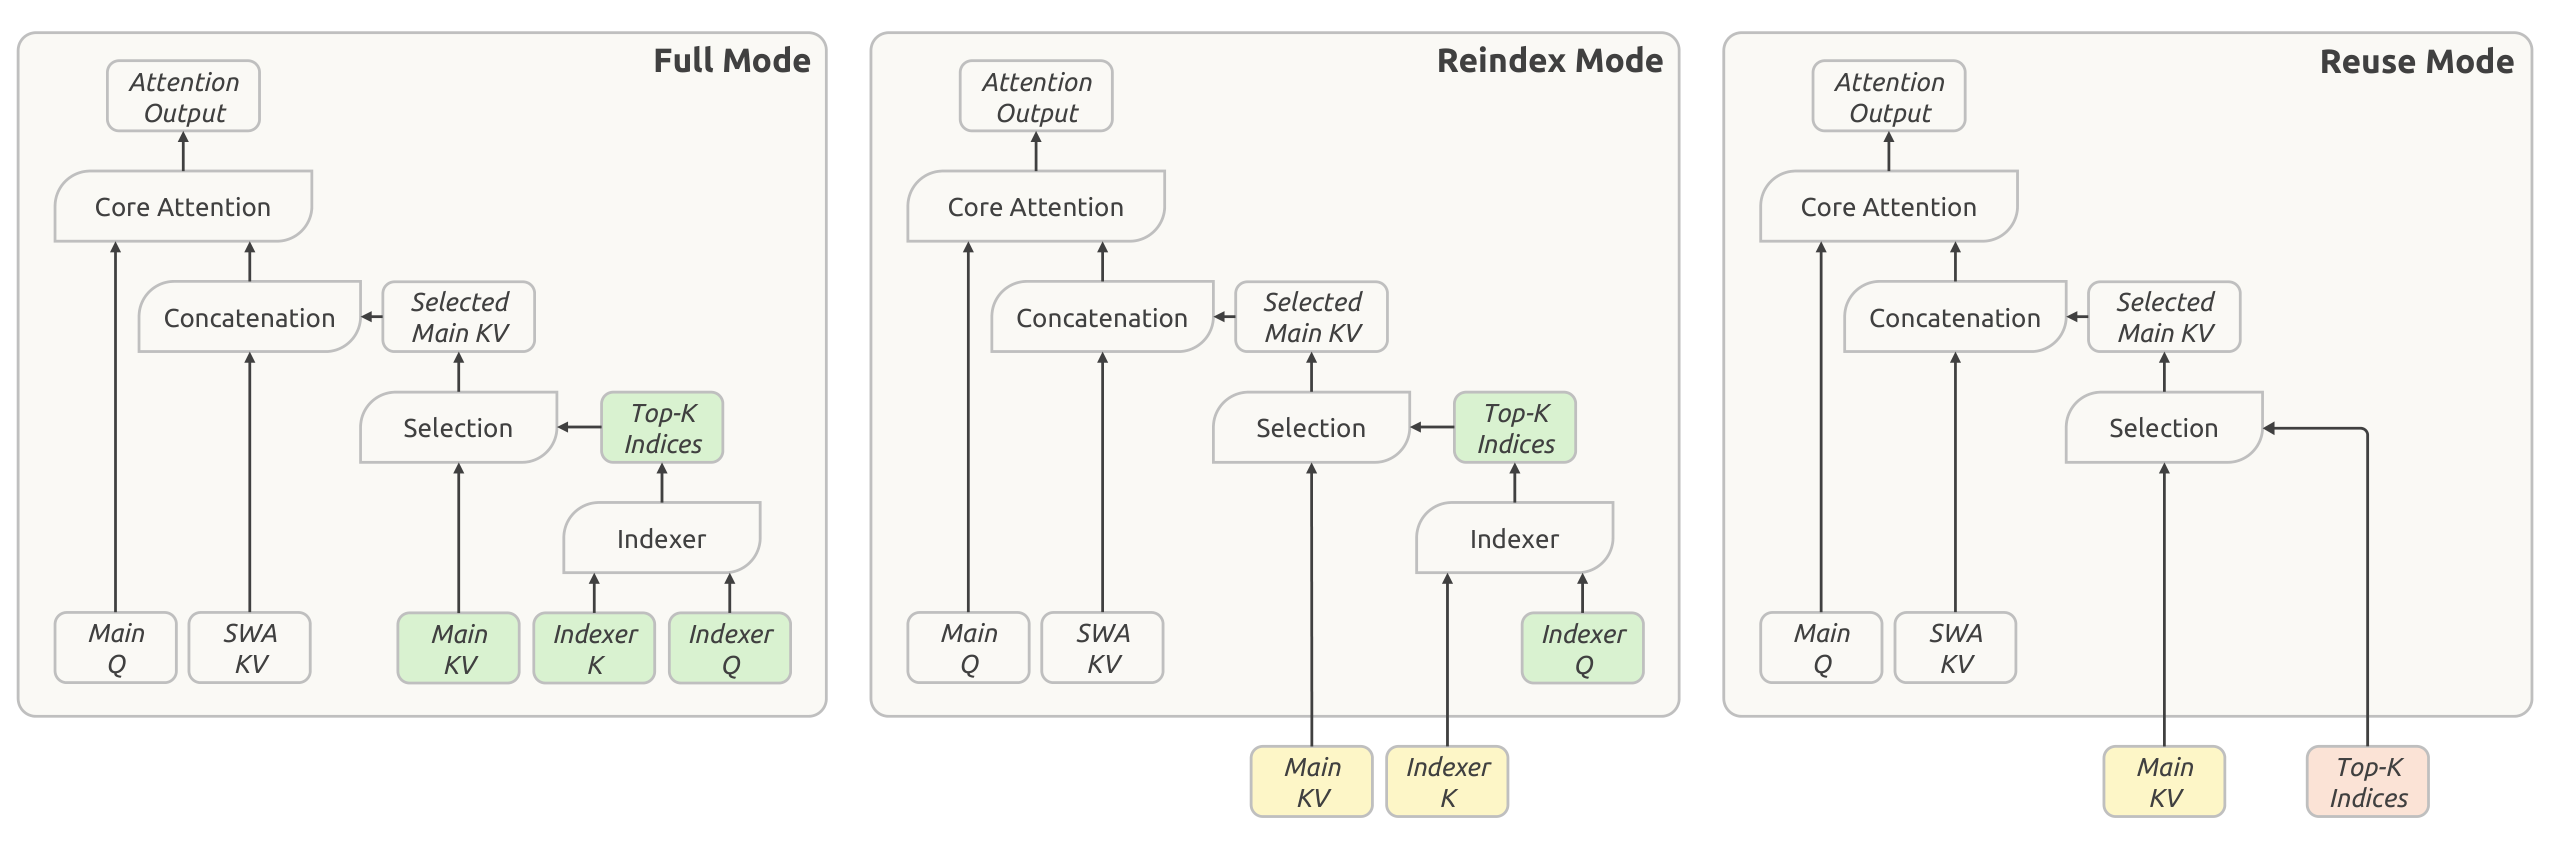
\includegraphics[width=\linewidth]{images_hi/fig04}
\caption{CSA2 的三种运行模式。这些模式在主 KV、索引器 K 和 Top-K 索引的获取方式上有所不同。绿色块表示在当前层中计算的量；黄色块表示从最近的 Full Mode 层复用的主 KV 和索引器 K；红色块表示从最近的生成索引的（Full Mode 或 Reindex Mode）层复用的 Top-K 索引。三种模式均会在当前层计算主 Q 和 SWA KV。}
\label{fig:4}
\end{figure}